\chapter{Introduction}
\label{cha:introduction}

\dictum[Rachel Carson, \textit{Silent Spring} (1962)]{%
  The balance of nature is not a status quo; it is fluid, ever shifting, in a constant state of adjustment. \\ Man, too, is part of this balance.}%
\vskip 1em


Biology is determined by structure, patterns, and dynamics at various scales, ranging from molecular interactions to organismal behavior.
%
% Recent technologies have provided access, with an unprecedented resolution, once deemed unthinkable, into the inner workings of cells and tissues that lie on the lower-end of that scale.
%
At the lower end of that scale, single-cell genomics and transcriptomics provide now a direct window, with a resolution that was deemed unthinkable two decades ago, into the molecular makeup of individual cells, capturing vividly the inner workings of cells at any point in time.
%paving the way for a better understanding of the diversity of cell types and their functional roles. 
Similarly, advances in imaging technology provide tools to map the spatial organization of tissues and organs at the cellular and subcellular level, improving our understanding of key physiological processes.% that underlie health and disease.
%
The ability of single-cell high-throughput methods to produce routinely millions of data points holds multiple promises. They do, however,  come with an important limitation: they produce data that are not \textit{aligned}, namely, such methods are destructive assays, meaning that the same cell cannot be observed twice.
% nor fully profiled over time.
% Since many of the most pressing questions in the field involve modeling and understanding the dynamic responses of heterogeneous cell populations to various stimuli, such as environmental signals, developmental processes, genetic perturbations, or drug treatments, there is a pressing need to provide experimental and/or computational methods that can circumvent that limitation. 
This limitation is particularly acute in the field of personalized medicine, where the goal is precisely to understand the dynamic response of a patient's cells to a stimulus, and would therefore rest, in theory, on the ability to observe the same cell before and after treatment.
%
Similarly, most single-cell technologies require the physical dissection and dissociation of tissues and organs, resulting in a loss of spatial information.
%
These issues are well known challenges, and many technologies have tried to circumvent such destructive steps, notably through spatial-omics. The scalability of such methods does, however, lag behind that of single-cell sequencing, which calls for algorithmic solutions to this problem.


Our goal in this review is to highlight that the common thread in all of these problems is the recurring need to realign datasets, and that such problems can be solved using optimal transport (OT) theory \citep{villani2021topics, santambrogio2015optimal}.
OT theory, a major research area in pure mathematics in recent decades (with Fields Medals awarded to \citeauthor{villani2021topics} in 2010 and \citeauthor{figalli2017monge} in 2018), has emerged as a contender to fill in that gap \textit{in silico}. OT is best described as a toolbox that allows reconstructing how a \emph{source} population (represented as one probability distribution) can morph efficiently into another \emph{target} population, given only source and target samples. Taking for the source distribution a sample of cells pre-stimuli, and for the target, another sample of cells post-stimuli, OT can reconstruct the unobserved process and provide an informed guess to define a \emph{transport map} that relates these two cell populations. 

\begin{figure}[t]
  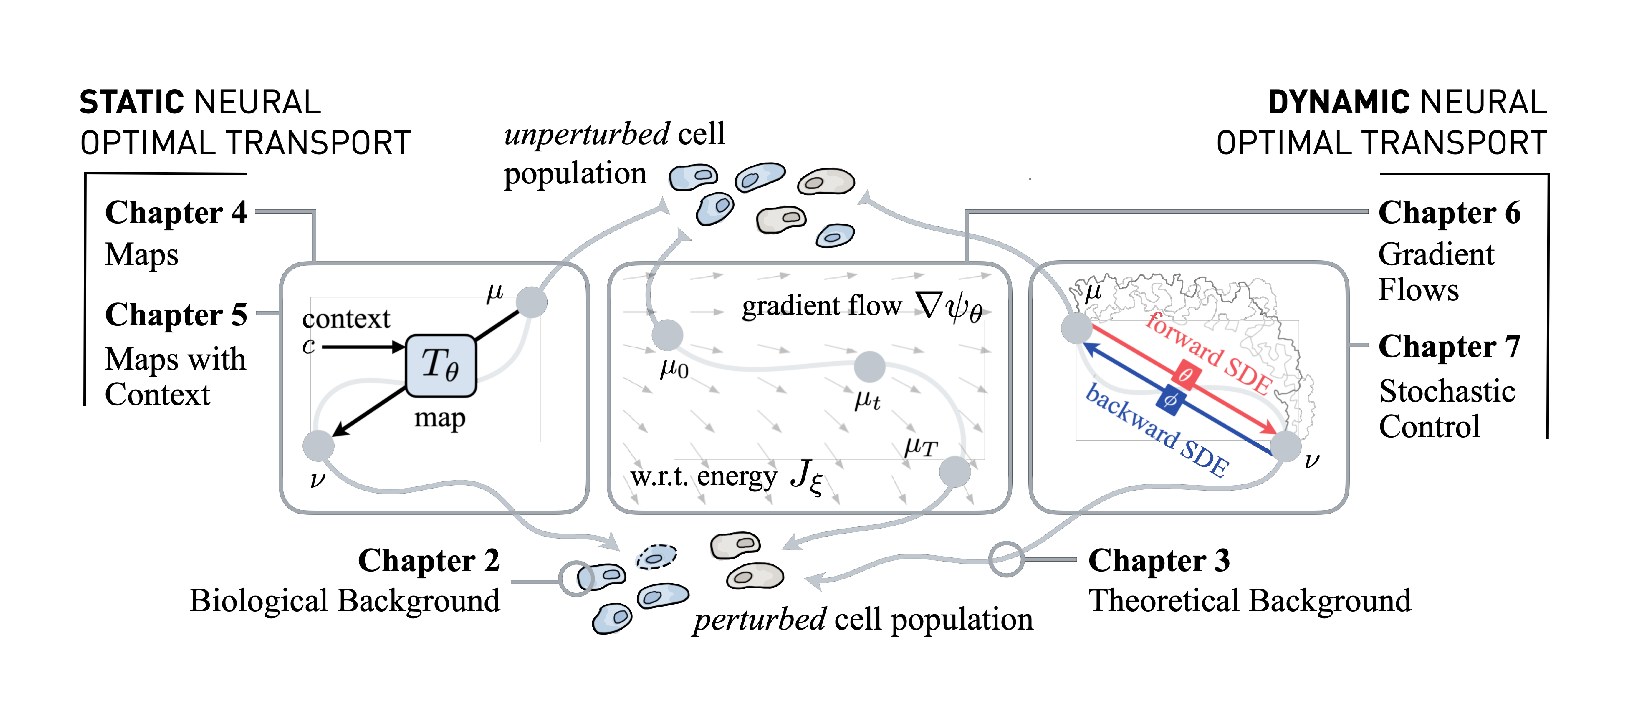
\includegraphics[width=\textwidth]{figures/fig_overview_thesis.pdf}
  \caption{Overview on ...}
\end{figure}


Applied to the analysis and modeling of single-cell biology problems, OT has been used to infer the distributions of cells' ancestors and descendants along development \citep{schiebinger2019optimal}, perform trajectory inference \citep{bunne2022proximal, forrow2021lineageot, bunne2022recovering, lavenant2021towards, schiebinger2019optimal, tong2020trajectorynet, yang2020predicting, zhang2021optimal, chizat2022trajectory}, predict perturbation responses \citep{bunne2021learning, yang2018scalable, lubeck2022neural}, integrate multi-omics data of different modalities \citep{demetci2022scot}, infer cell-cell similarity \citep{huizing2022optimal}, and integrate across scales (e.g., morphology and molecular profiling) \citep{yang2021multi}. The increasing data complexity across multiple levels of biological organization, from molecular and cellular through spatial profiling \citep{moriel2021novosparc} of tissues, and imaging of organs, cement further the status of OT as an indispensable framework for high-throughput, multimodal, and multi-scale molecular, cell, tissue, and organ biology. The effectiveness of OT comes, however, with drawbacks: because the theory builds on extremely sophisticated mathematics that blends optimization \citep{cuturi2013sinkhorn, cuturi2022optimal}, stochasticity \citep{chizat2022trajectory, bunne2022recovering} and partial differential equations \citep{bunne2022proximal}, and, more recently, deep learning \citep{tong2020trajectorynet, bunne2021learning, bunne2022supervised, yang2018scalable, lubeck2022neural, yang2021multi}, its computations are challenging even by modern ML standards.

% By leveraging the principles of optimal transport, ... and thus overcome the limitations of traditional methods and unlock new insights into the complexity of biological systems.
% ...

In this primer, we introduce the mathematical and computational principles of OT, with the goal of facilitating its use by researchers that wish to apply to novel applications. We provide the reader with intuitive explanations of how seemingly unrelated mathematical approaches for analyzing single-cell data can be unified through OT theory, and how that theory has triggered recent advances in deep learning. We provide an overview of the broad range of biological applications, demonstrating the successes of OT in the field, especially within the field of single-cell biology. With its rich properties, astonishing mathematical connections, and its innovative numerical implementations \citep{cuturi2022optimal}, OT makes for an exciting avenue of future work to make novel biological discoveries, infer personalized cancer therapies from single-cell patient samples, and push the boundaries of regenerative medicine.

\section{Contributions}


\section{Thesis Organization}

This thesis is organized in two parts. \cref{part:static_not} is dedicated to introducing static neural optimal transport methods and comprises two chapters:
\cref{cha:cellot} .... To ..., \cref{cha:condot} ...

\cref{part:dynamic_not} subsequently covers methods within the dynamic neural optimal transport framework. In particular, \cref{cha:neural_pde} ...
\cref{cha:neural_sde} ...
\cref{sec:gsbflow} ... \cref{sec:sb_align} ...


\section{Publications}
All results presented in this thesis have been published in the following conference proceedings and journals:

\begin{itemize}
	\item[] Charlotte Bunne, Laetitia Meng-Papaxanthos, Andreas Krause, and Marco Cuturi. Proximal Optimal Transport Modeling of Population Dynamics. In \textit{International Conference on Artificial Intelligence and Statistics (AISTATS)}, volume 25, 2022.
	\item[] Charlotte Bunne, Andreas Krause, and Marco Cuturi. Supervised Training of Conditional Monge Maps. In \textit{Advances in Neural Information Processing Systems (NeurIPS)}, 2022.
	\item[] Charlotte Bunne, Ya-Ping Hsieh, Marco Cuturi, and Andreas Krause. The Schr{\"o}dinger Bridge between Gaussian Measures has a Closed Form. In \textit{International Conference on Artificial Intelligence and Statistics (AISTATS)}, 2023.
	\item[] Vignesh Ram Somnath, Matteo Pariset, Ya-Ping Hsieh, Maria Rodriguez Martinez, Andreas Krause, and Charlotte Bunne. Aligned Diffusion Schr{\"o}dinger Bridges. In \textit{Conference on Uncertainty in Artificial Intelligence (UAI)}, 2023.
	\item[] Charlotte Bunne, Stefan G Stark, Gabriele Gut, Jacobo Sarabia del Castillo, Kjong-Van Lehmann, Lucas Pelkmans, Andreas Krause, and Gunnar R{\"a}tsch. Learning Single-Cell Perturbation Responses using Neural Optimal Transport. \textit{Nature Methods}, 2023.
\end{itemize}

\paragraph{Further publications.}
The following publications of the author and collaborators are more broadly relevant to the topic of this thesis but have not been directly included:

\begin{itemize}
	\item[] Charlotte Bunne, David Alvarez-Melis, Andreas Krause, and Stefanie Jegelka. Learning Generative Models across Incomparable Spaces. In \textit{International Conference on Machine Learning (ICML)}, 2019.
	\item[] Vignesh Ram Somnath, Charlotte Bunne, Connor Coley, Andreas Krause, and Regina Barzilay. Learning Graph Models for Retrosynthesis Prediction. In Advances in Neural Information Processing Systems (NeurIPS), 2021.
	\item[] Vignesh Ram Somnath, Charlotte Bunne, and Andreas Krause. Multi-Scale Representation Learning on Proteins. In \textit{Advances in Neural Information Processing Systems (NeurIPS)}, 2021.
	\item[] Marco Cuturi, Laetitia Meng-Papaxanthos, Yingtao Tian, Charlotte Bunne, Geoff Davis, and Olivier Teboul. Optimal Transport Tools (OTT): A JAX Toolbox for all things Wasserstein. \textit{arXiv Preprint arXiv: 2201.12324}, 2022.
	\item[] Octavian-Eugen Ganea, Xinyuan Huang, Charlotte Bunne, Yatao Bian, Regina Barzilay, Tommi S. Jaakkola, and Andreas Krause. Indepen- dent SE(3)-Equivariant Models for End-to-End Rigid Protein Docking. In \textit{International Conference on Learning Representations (ICLR)}, 2022.
	\item[] Philippe Schwaller, Alain C Vaucher, Ruben Laplaza, Charlotte Bunne, Andreas Krause, Clemence Corminboeuf, and Teodoro Laino. Machine intelligence for chemical reaction space. \textit{Wiley Interdisciplinary Reviews: Computational Molecular Science}, 2022.
	\item[] Frederike L\"ubeck, Charlotte Bunne, Gabriele Gut, Jacobo Sarabia del Castillo, Lucas Pelkmans, and David Alvarez-Melis. Neural Unbalanced Optimal Transport via Cycle-Consistent Semi-Couplings. \textit{arXiv Preprint arXiv: 2209.15621}, 2022.
	\item[] Matteo Pariset, Ya-Ping Hsieh, Charlotte Bunne, Andreas Krause, and Valentin De Bortoli. Unbalanced Diffusion Schr{\"o}dinger Bridge. \textit{arXiv Preprint arXiv: 2306.09099}, 2023
\end{itemize}

\section{Collaborators}

This thesis would not have been possible without my advisors, Andreas Krause and Marco Cuturi, and many of the ideas presented here have been shaped in our meetings. I further enjoyed collaborating with my colleagues on numerous ideas and the results presented and not otherwise cited are by the author and collaborators. In particular, \cref{cha:cellot} contains material of a publication with shared first authorship between the author, Stefan Stark, and Gabriele Gut. Besides Andreas Krause, Kjong-Van Lehmann, Lucas Pelkmans, and Gunnar R\"atsch serve as corresponding authors.
\cref{sec:gsbflow} is based on a joint first authorship project with Ya-Ping Hsieh who contributed the theoretical analysis of that work. Lastly, \cref{sec:sb_align} contains material from a publication where Vignesh Ram Somnath and Matteo Pariset share the first authorship while the author serves as corresponding author.

